\chapter{História}
\label{cap.historia}
\paragraph{}
\section{História}
	A cada dia que passa, esta tecnologia avança cada vez mais, e atualmente já é possivel retirarmos proveito de diversas maneiras deste conceito de realidade virtual.Esta foi um objeto de estudo durante vários anos, e foi progredindo de forma lenta e pouco regular, sendo a sua grande expansão, apenas na última década.
	\subsection{Estereoscópio - 1838}
		\paragraph{}
Ao que tudo indica, o pioneiro desta tecnologia foi Sir Charles Wheatstone que inventou o Estereoscópio, um aparelho de análise de diversas imagens em diferentes perspectivas com o objetivo de oferecer a ilusão de uma vista tridimensional.
			\begin{figure}
				\center
%				\includegraphics[scale=0.3]{imagens/Estereoscópio.jpg}
				\caption{Estereoscópio \cite{4}}
			\end{figure}
	\subsection{\textit{Pygmalion’s Spectacles - 1935}}
	\paragraph{}
Escrito por Stanley G. Weinbaum a 1935,  \textit{Pygmalion's Spectacles} é uma pequena história onde o protagonista conhece um professor que inventa uns óculos que permitiam a uma pessoa sentir-se dentro do filme que estão a ver, algo muito parecido com o que no futuro se tornou a realidade virtual.
	\subsection{Sensorama - 1955}
 \paragraph{}
 Foi então em 1955 que o pioneiro nesta tecnologia, Morton Heilig, visionou, e mais tarde em 1962 acabou por o desenvolver, o primeiro projeto de realidade virtual como nós a conhecemos .
 
O Sensorama é uma máquina que tem como propósito a reprodução de filmes acompanhados dos mais diversos efeitos sensoriais de maneira a criar imersão ao utilizador.Servia-se de uma visão de imagens estereoscopicas em 3D , combinado com um movimento do corpo,cheiros e vento de acordo com o ambiente da imagem e sons em \textit{stereo} durante a reprodução do filme(Uma versão mais primitiva do que se intitula nos dias de hoje de: Cinema 4D).

Apesar de todo o sucesso, Heilig não foi capaz de obter apoio financeiro para as suas patentes, o que obrigou o término deste projeto.
	\begin{figure}
	\center
	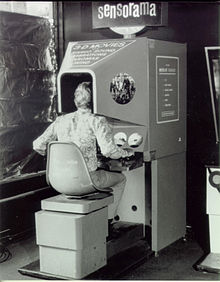
\includegraphics[scale=0.5]{imagens/Sensorama.jpg}
	\caption{Sensorama. \cite{5}}
	\end{figure}
	\subsection{Headsight - 1961}
	\paragraph{}
Headsight foi o primeiro HMD a integrar sensores de movimento."É constituido por um ecrã para cada olho e por um sensor de movimentos conectado a uma câmera por um circuito fechado.Ao contrário do que pode parecer, nao foi desenvolvida com propósitos de Realidade Virtual, mas para efeitos militares,cujo objetivo seria visualizar os perigos de certas situações."\cite{10}
	
	\subsection{Ultimate Display - 1965 / Sword of Damocles - 1968}
\paragraph{}
Seguindo a ideia por trás do Sensorama, Ivan Sutherland escreve o artigo: \textit{The Ultimate Display}, que revolucionou o pensamento da época e acabou por impulsionar a ideia de Realidade Virtual.Sutherland disserta sobre a ideia da evolução tecnológica e do seu potencial e limites,referindo que "um computador não tem de se limitar ás leis da fisica tal como nós"\cite{11}, admitindo por fim, que o \textit{"auge da tecnologia(\textbf{ Ultimate Display}) seria um computador capaz de alterar toda a matéria numa sala , incluindo gerar cadeiras que seriam possiveis de se sentar , algemas que conseguiriam prender e balas que poderiam ser fatais.Com a programação certa, este dispositivo poderia ser literalmente o País das Maravilhas em que a Alice entrou "}\cite{11}.

Poucos anos mais tarde , este mesmo senhor desenvolveu um protótipo bastante rudimentar este artigo, ao qual intitulou de "\textit{Sword of Damocles}".Este dispositivo ainda ficava muito aquém, tanto na interface de usuário como no grafismo da aplicação.Semelhante ao Sensorama,o sistema de reprodução era feito entre o computador e um ecrã estereoscópico.Continha um sensor de movimento no HMD, o que juntamente com o estereoscópio, que permitia o ecrã ajustar-se á posição da pessoa.

A primeira aplicação a ser desenvolvida para este aparelho, era um cubo suspenso por um fio, em frente ao utilizador e era composto por uma série de diversos hardwares.Esta ideia foi inspirada na história do nome do próprio aparelho:"\textit{Sword of Damocles}", que nos conta uma breve história sobre Damocles, um homem do povo ao qual foi dada a proposta que poderia ser rei por um dia, mas teria uma espada presa por apenas um fio de cabelo de um cavalo por cima do seu trono. 
\begin{figure}
\center
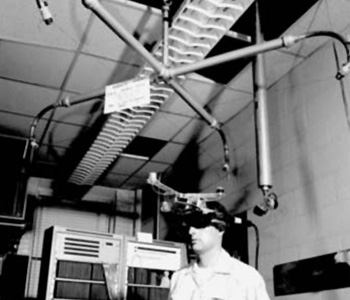
\includegraphics[scale=0.4]{imagens/SOD.jpg}
\caption{Sword of Damocles -  Era uma máquina intimidante e pouco prática. \cite{6}}
\end{figure}
	\subsection{Realidade Artificial - 1969}
\paragraph{}
Myron Kruegere , um artista de realidade virtual, conduziu uma série de testes na tentativa bem sucedida de criar um mundo que interagisse e respondesse ás ações do usuário.Através desta tecnologia , era possivel as pessoas comunicarem umas com as outras num ambiente gerado por um computador.
	\subsection{O nascimento do nome - 1987}
\paragraph{}
Apesar de toda esta tecnologia, ainda não existia um termo que associasse e unisse toda esta tecnologia.Jaron Lanier apelidou então, em 1987, este campo de "Realidade Virtual".
	
A sua empresa começou então a desenvolver equipamentos para esta área, tais como luvas e óculos.
	\subsection{Consumo Público - 1991}
\paragraph{}
Foi na década de oitenta e noventa que a Realidade Virtual começou a ganhar força, no entanto ainda estava bastante inacessivel para uma utilização caseira.Chega-nos consequentemente o lançamento de máquinas de jogos arcade de RV pelo TVG. Os jogadores utilizariam um par de óculos e disfrutavam do jogo em tempo real, e alguns desses jogos até chegavam a estar conectados numa rede para incluir um modo multi jogador.
\begin{figure}
\center
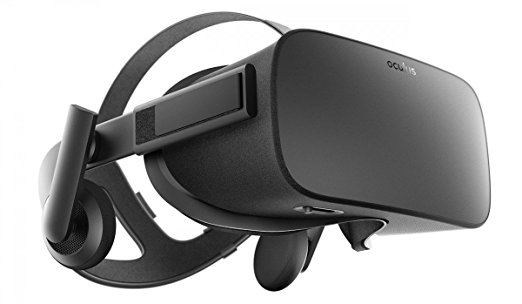
\includegraphics[scale=0.3]{imagens/OR.jpg}
\caption{Oculus Rift}
\end{figure}
\subsection{Inicio das consolas VR - 1993}
\paragraph{}
Em 1993, a SEGA lançou um novo produto de óculos de RV para a sua consola SEGA Genesis.Estes óculos disfrutavam de sensor de movimento, som em \textit{stereo} e um ecrã em LCD. Infelizmente, devido a problemas técnicos e apesar de terem sido lançados 4 jogos para esta plataforma, a mesma nunca chegou a passar de uma fase de protótipo.
\subsection{Realidade Virtual nos dias de hoje}
\paragraph{}
Ninguém pode negar que o crescimento da Realidade Virtual tem sido exponencial, e começou o seu grande desenvolvimento no séc. XXI.A tecnologia dos computadores é cada vez mais avançada e a acessibilidade dos produtos ao consumidor é cada vez mais facil.A evolução dos smartphones contribuiu bastante também para a explosão da Realidade Virtual, pois permite-nos ter dispositivos portáteis com bastante capacidade e potência, nunca deixando de ser leves e de boa mobilidade.Enquanto isso, a industria dos video-jogos continua o seu desenvolvimento, sempre na liderança da utilização desta tecnologia.

Muitas empresas estão a começar a investir nesta área, tais como a Google que desenvolve headsets controlados por smarthphones, a Samsung que implementa novas funções de realidade virtual a cada produto Galaxy que lançam, e até mesmo o Facebook, o que começou como uma rede social , chegou mesmo a comprar os direitos dos Oculus Rift, um dos HMDs mais populares da atual geração, competindo com grandes nomes da área de entertenimento como a Valve, Microsoft e Sony.




